\documentclass[12pt]{article}
\usepackage[a4paper, top=0.8in, bottom=0.7in, left=0.8in, right=0.8in]{geometry}
\usepackage{amsmath, amsfonts, graphicx, fancyhdr, enumitem, setspace, tcolorbox, tikz, xcolor}
\usepackage[defaultfam,tabular,lining]{montserrat}
\renewcommand*\oldstylenums[1]{{\fontfamily{Montserrat-TOsF}\selectfont #1}}
\renewcommand{\familydefault}{\sfdefault}

\setlength{\headheight}{27.11148pt} 

\setlength{\parindent}{0pt}
\pagestyle{fancy}
\fancyhf{}
\fancyhead[L]{Practice Exam G - ANSWER KEY}
\fancyhead[R]{
\includegraphics[width=0.8cm]{Round Logo.png}}
\fancyfoot[C]{\footnotesize © Study Smart Tutors}

\begin{document}

\subsection*{Assessment G: Math Pre/Post-Assessment - ANSWER KEY}
\onehalfspacing

\begin{tcolorbox}[colframe=black!50, colback=white, title=Assessment Directions]
\textbf{Directions:} Solve each question carefully. For multiple-choice questions, circle the correct answer. For written responses, show your work and explain your reasoning.
\end{tcolorbox}

% Problem 1
\begin{tcolorbox}[colframe=black!50, colback=white, title=\textbf{Problem 1 (6.EE.A.2)}]
Write an expression for the following scenario: 

``Twice the sum of a number \(x\) and 5.'' 

\textbf{Answer:} \textcolor{red}{\(2(x + 5)\)}  
\textcolor{red}{Explanation: The sum of \(x\) and 5 is written as \(x + 5\). Multiplying it by 2 gives \(2(x + 5)\).}
\end{tcolorbox}

% Problem 2
\begin{tcolorbox}[colframe=black!50, colback=white, title=\textbf{Problem 2 (6.RP.A.1)}]
The ratio of boys to girls in a classroom is \(3:2\). Which of the following statements is correct?

\textbf{Answer Options:}
\begin{enumerate}[label=(\Alph*), itemsep=0.5cm]
    \item There are 3 boys for every 2 girls.
    \item The number of boys is twice the number of girls.
    \item The number of girls is greater than the number of boys.
    \item For every 5 students, there are 2 girls.
\end{enumerate}
\textbf{Answer:} \textcolor{red}{(A)}  
\textcolor{red}{Explanation: A ratio of \(3:2\) means that for every 3 boys, there are 2 girls.}
\end{tcolorbox}

% Problem 3
\begin{tcolorbox}[colframe=black!50, colback=white, title=\textbf{Problem 3 (6.NS.C.6)}]
On a number line, plot the points \(-2.5\), \(0\), and \(3.5\). Label each point clearly.

\begin{center}
    \begin{tikzpicture}[x=1cm, y=1cm]
        % Number line
        \draw[thick, ->] (-3.5,0) -- (4.5,0);
        \foreach \x in {-3,-2,-1,0,1,2,3,4} {
            \draw[thick] (\x,0.1) -- (\x,-0.1);
            \node[below] at (\x, -0.2) {\x};
        }
        % Points
        \filldraw[red] (-2.5,0) circle (0.1cm) node[above] {\(-2.5\)};
        \filldraw[red] (0,0) circle (0.1cm) node[above] {0};
        \filldraw[red] (3.5,0) circle (0.1cm) node[above] {\(3.5\)};
    \end{tikzpicture}
\end{center}
\textcolor{red}{Explanation: Points are plotted at the correct positions on the number line.}
\end{tcolorbox}

% Problem 4
\begin{tcolorbox}[colframe=black!50, colback=white, title=\textbf{Problem 4 (6.EE.B.5)}]
Which of the following values makes the inequality \(2x + 4 > 10\) true?

\textbf{Answer Options:}
\begin{enumerate}[label=(\Alph*), itemsep=0.5cm]
    \item \(x = 1\)
    \item \(x = 2\)
    \item \(x = 3\)
    \item \(x = 4\)
\end{enumerate}
\textbf{Answer:} \textcolor{red}{(D)}  
\textcolor{red}{Explanation: Solve \(2x + 4 > 10 \implies 2x > 6 \implies x > 3\). The smallest value of \(x > 3\) is 4.}
\end{tcolorbox}

% Problem 5
\begin{tcolorbox}[colframe=black!50, colback=white, title=\textbf{Problem 5 (6.NS.A.1)}]
Divide \(\frac{3}{4} \div \frac{1}{2}\). Use a visual fraction model to explain your answer.

\textbf{Answer:} \textcolor{red}{\(\frac{3}{4} \div \frac{1}{2} = \frac{3}{4} \times 2 = \frac{6}{4} = 1\frac{1}{2}\)}  
\textcolor{red}{Explanation: Dividing by a fraction is the same as multiplying by its reciprocal.}
\end{tcolorbox}

% Problem 6
\begin{tcolorbox}[colframe=black!50, colback=white, title=\textbf{Problem 6 (6.RP.A.2)}]
Find the unit rate: \(12\) oranges cost \(\$4.80\). What is the cost per orange?

\textbf{Answer:} \textcolor{red}{\(\frac{4.80}{12} = 0.40\)}  
\textcolor{red}{Explanation: Divide total cost by total oranges to find the cost per orange.}
\end{tcolorbox}

% Problem 7
\begin{tcolorbox}[colframe=black!50, colback=white, title=\textbf{Problem 7 (6.NS.C.7)}]
Order the following numbers from least to greatest: \(-3.2, 0, 2.5, -1.8\).

\textbf{Answer:} \textcolor{red}{\(-3.2, -1.8, 0, 2.5\)}  
\textcolor{red}{Explanation: Compare the values and arrange them on a number line.}
\end{tcolorbox}

% Problem 8
\begin{tcolorbox}[colframe=black!50, colback=white, title=\textbf{Problem 8 (6.RP.A.3)}]
A recipe calls for 4 cups of flour to make 8 cookies. How much flour is needed to make 20 cookies?

\textbf{Answer:} \textcolor{red}{\(\frac{20}{8} \times 4 = 10 \text{ cups}\)}  
\textcolor{red}{Explanation: The recipe scales proportionally.}
\end{tcolorbox}

% Problem 9
\begin{tcolorbox}[colframe=black!50, colback=white, title=\textbf{Problem 9 (6.NS.A.1)}]
Solve the word problem: Sarah has \(\frac{2}{3}\) of a cake. She gives \(\frac{1}{4}\) of the cake to her friend. How much cake does she have left?

\textbf{Answer:} \textcolor{red}{\(\frac{2}{3} - \frac{1}{4} = \frac{8}{12} - \frac{3}{12} = \frac{5}{12}\)}  
\textcolor{red}{Explanation: Use a common denominator to subtract fractions.}
\end{tcolorbox}

% Problem 10
\begin{tcolorbox}[colframe=black!50, colback=white, title=\textbf{Problem 10 (6.NS.C.8)}]
Graph the points \((-2, 4)\), \((3, 4)\), and \((0, 0)\) on the coordinate plane. Find the distance between \((-2, 4)\) and \((3, 4)\).

\begin{center}
    \begin{tikzpicture}[scale=0.8]
        % Draw grid
        \draw[step=1cm, gray!30, very thin] (-5.5,-5.5) grid (5.5,5.5);

        % Draw axes
        \draw[thick, ->] (-5.5,0) -- (5.5,0) node[right] {\(x\)};
        \draw[thick, ->] (0,-5.5) -- (0,5.5) node[above] {\(y\)};

        % Label ticks on x-axis
        \foreach \x in {-5,-4,-3,-2,-1,1,2,3,4,5} {
            \draw[thick] (\x,0.1) -- (\x,-0.1) node[below] {\(\x\)};
        }

        % Label ticks on y-axis
        \foreach \y in {-5,-4,-3,-2,-1,1,2,3,4,5} {
            \draw[thick] (0.1,\y) -- (-0.1,\y) node[left] {\(\y\)};
        }

        % Points
        \filldraw[red] (-2,4) circle (0.1cm) node[above left] {\((-2, 4)\)};
        \filldraw[red] (3,4) circle (0.1cm) node[above right] {\((3, 4)\)};
        \filldraw[red] (0,0) circle (0.1cm) node[below right] {\((0, 0)\)};
    \end{tikzpicture}
\end{center}
\textbf{Answer:} \textcolor{red}{Distance = \(3 - (-2) = 5\)}  
\textcolor{red}{Explanation: Subtract \(x\)-coordinates as the \(y\)-values are the same.}
\end{tcolorbox}

\end{document}
